\documentclass[12pt]{article}
\usepackage{graphicx}

\title{Longest Path MapReduce Implementation}
\author{}
\date{}

\begin{document}

\maketitle

\begin{abstract}
This report describes the implementation of the Longest Path problem using a Python-based MapReduce approach with Apache Spark. The program identifies the longest file path based on the number of '/' characters, representing the depth of a directory structure. The implementation leverages Spark's parallel processing capabilities to handle large datasets efficiently. Tasks were divided among five group members for collaborative work.
\end{abstract}

\section{Introduction}
The Longest Path problem is a distributed computing challenge where the goal is to identify the file path with the maximum depth in a directory structure. In this project, we implemented the solution using Apache Spark's MapReduce framework. Each file path is processed to compute its depth, and the longest path is identified across all files.

\subsection{Task Division}
The implementation tasks were divided among the team members as follows:
\begin{itemize}
    \item Vu Hai Thien Long: Designed and implemented the Mapper function to calculate the depth of each file path.
    \item Luu Linh Ly: Developed the Reducer function to group paths by depth and find the longest path.
    \item Nguyen Ngoc Nhi: Handled the integration of the Mapper and Reducer, ensuring the correct execution flow.
    \item Le Viet Hoang Lam: Created the functionality to write results to the output directory and formatted the output.
    \item Nguyen Duc Duy: Managed overall testing, debugging, and ensuring scalability for large datasets.
\end{itemize}

\section{Choice of MapReduce Framework}
We selected Apache Spark for its scalability and built-in support for distributed computing. Key motivations for this choice include:
\begin{itemize}
    \item \textbf{Ease of Use}: Spark provides a Python API (PySpark) for building MapReduce solutions.
    \item \textbf{Parallel Processing}: Spark efficiently processes large datasets by distributing tasks across multiple nodes.
    \item \textbf{Fault Tolerance}: Spark's architecture ensures reliability even in case of node failures.
    \item \textbf{Scalability}: The solution can handle large numbers of files and complex directory structures.
\end{itemize}

\section{Mapper and Reducer Design}

\subsection{Mapper}
The Mapper processes each input file path to compute its depth (number of '/' characters) and emits a key-value pair:
\begin{itemize}
    \item \textbf{Key}: Depth (number of '/' characters).
    \item \textbf{Value}: Full file path.
\end{itemize}

\noindent Python code for the Mapper:
\begin{verbatim}
def mapper(line):
    path = line.strip()  # Remove whitespace
    depth = path.count('/')  # Count '/' characters
    return (depth, path)
\end{verbatim}

\subsection{Reducer}
The Reducer groups paths by depth and selects the longest path for each group. It then identifies the longest path with the maximum depth.

\noindent Python code for the Reducer:
\begin{verbatim}
def reducer(a, b):
    # Retain the longest path
    return a if len(a) >= len(b) else b
\end{verbatim}

\section{Flowchart of the Process}
Below is the flowchart illustrating the MapReduce process for solving the Longest Path problem:


\begin{figure}[h]
\centering
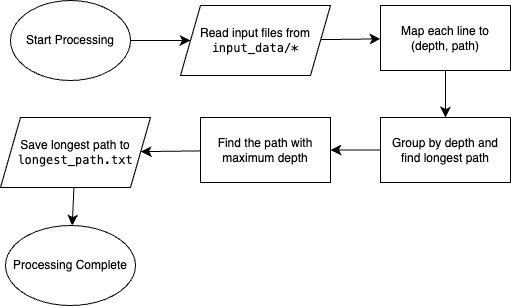
\includegraphics[width=0.6\textwidth]{mapper_reducer_workflow.png}
\caption{MapReduce Process for Longest Path}
\end{figure}

\section{Conclusion}
This implementation demonstrates the effectiveness of Apache Spark's MapReduce framework for solving the Longest Path problem. The Mapper efficiently calculates the depth of each file path, while the Reducer identifies the longest path with maximum depth.

\end{document}
